% Created 2024-06-29 Sat 09:30
% Intended LaTeX compiler: pdflatex
\documentclass[11pt]{article}
\usepackage[utf8]{inputenc}
\usepackage{lmodern}
\usepackage[T1]{fontenc}
\usepackage[top=1in, bottom=1.in, left=1in, right=1in]{geometry}
\usepackage{graphicx}
\usepackage{longtable}
\usepackage{float}
\usepackage{wrapfig}
\usepackage{rotating}
\usepackage[normalem]{ulem}
\usepackage{amsmath}
\usepackage{textcomp}
\usepackage{marvosym}
\usepackage{wasysym}
\usepackage{amssymb}
\usepackage{amsmath}
\usepackage[theorems, skins]{tcolorbox}
\usepackage[version=3]{mhchem}
\usepackage[numbers,super,sort&compress]{natbib}
\usepackage{natmove}
\usepackage{url}
\usepackage[cache=false]{minted}
\usepackage[strings]{underscore}
\usepackage[linktocpage,pdfstartview=FitH,colorlinks,
linkcolor=blue,anchorcolor=blue,
citecolor=blue,filecolor=blue,menucolor=blue,urlcolor=blue]{hyperref}
\usepackage{attachfile}
\usepackage{setspace}
\author{John Kitchin}
\date{\today}
\title{}
\begin{document}

\tableofcontents

\section{Electronic lab notebook with scimax - Remote Raspberry Pi by REST API}
\label{sec:org43c48ab}

\textit{{[}2024-06-26 Wed] } I made a video of this, but there were a bunch of technical difficulties, so I want to try making it again.

\begin{center}
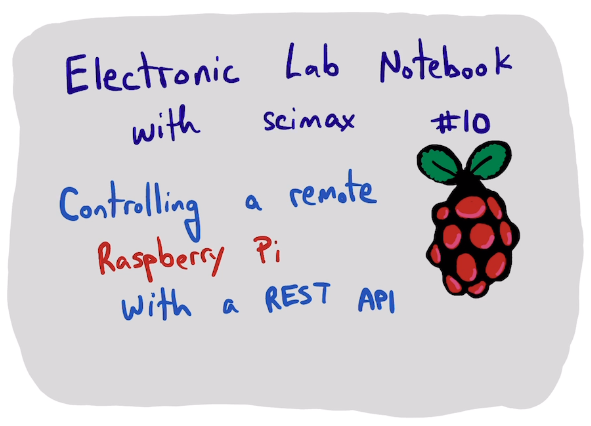
\includegraphics[width=.9\linewidth]{./screenshots/date-26-06-2024-time-15-15-46.png}
\end{center}
\section{In a browser}
\label{sec:org633f68f}

\url{http://arnold.wifi.local.cmu.edu:8080/img}
\section{In a shell}
\label{sec:org5260150}

\begin{minted}[frame=lines,fontsize=\scriptsize,linenos=]{sh}
curl http://arnold.wifi.local.cmu.edu:8080/img --output 3.59.jpg
\end{minted}
\section{in a sh src block}
\label{sec:org8a1fe31}

\begin{minted}[frame=lines,fontsize=\scriptsize,linenos=]{sh}
curl http://arnold.wifi.local.cmu.edu:8080/img --output 4.01.jpg
\end{minted}

\begin{center}
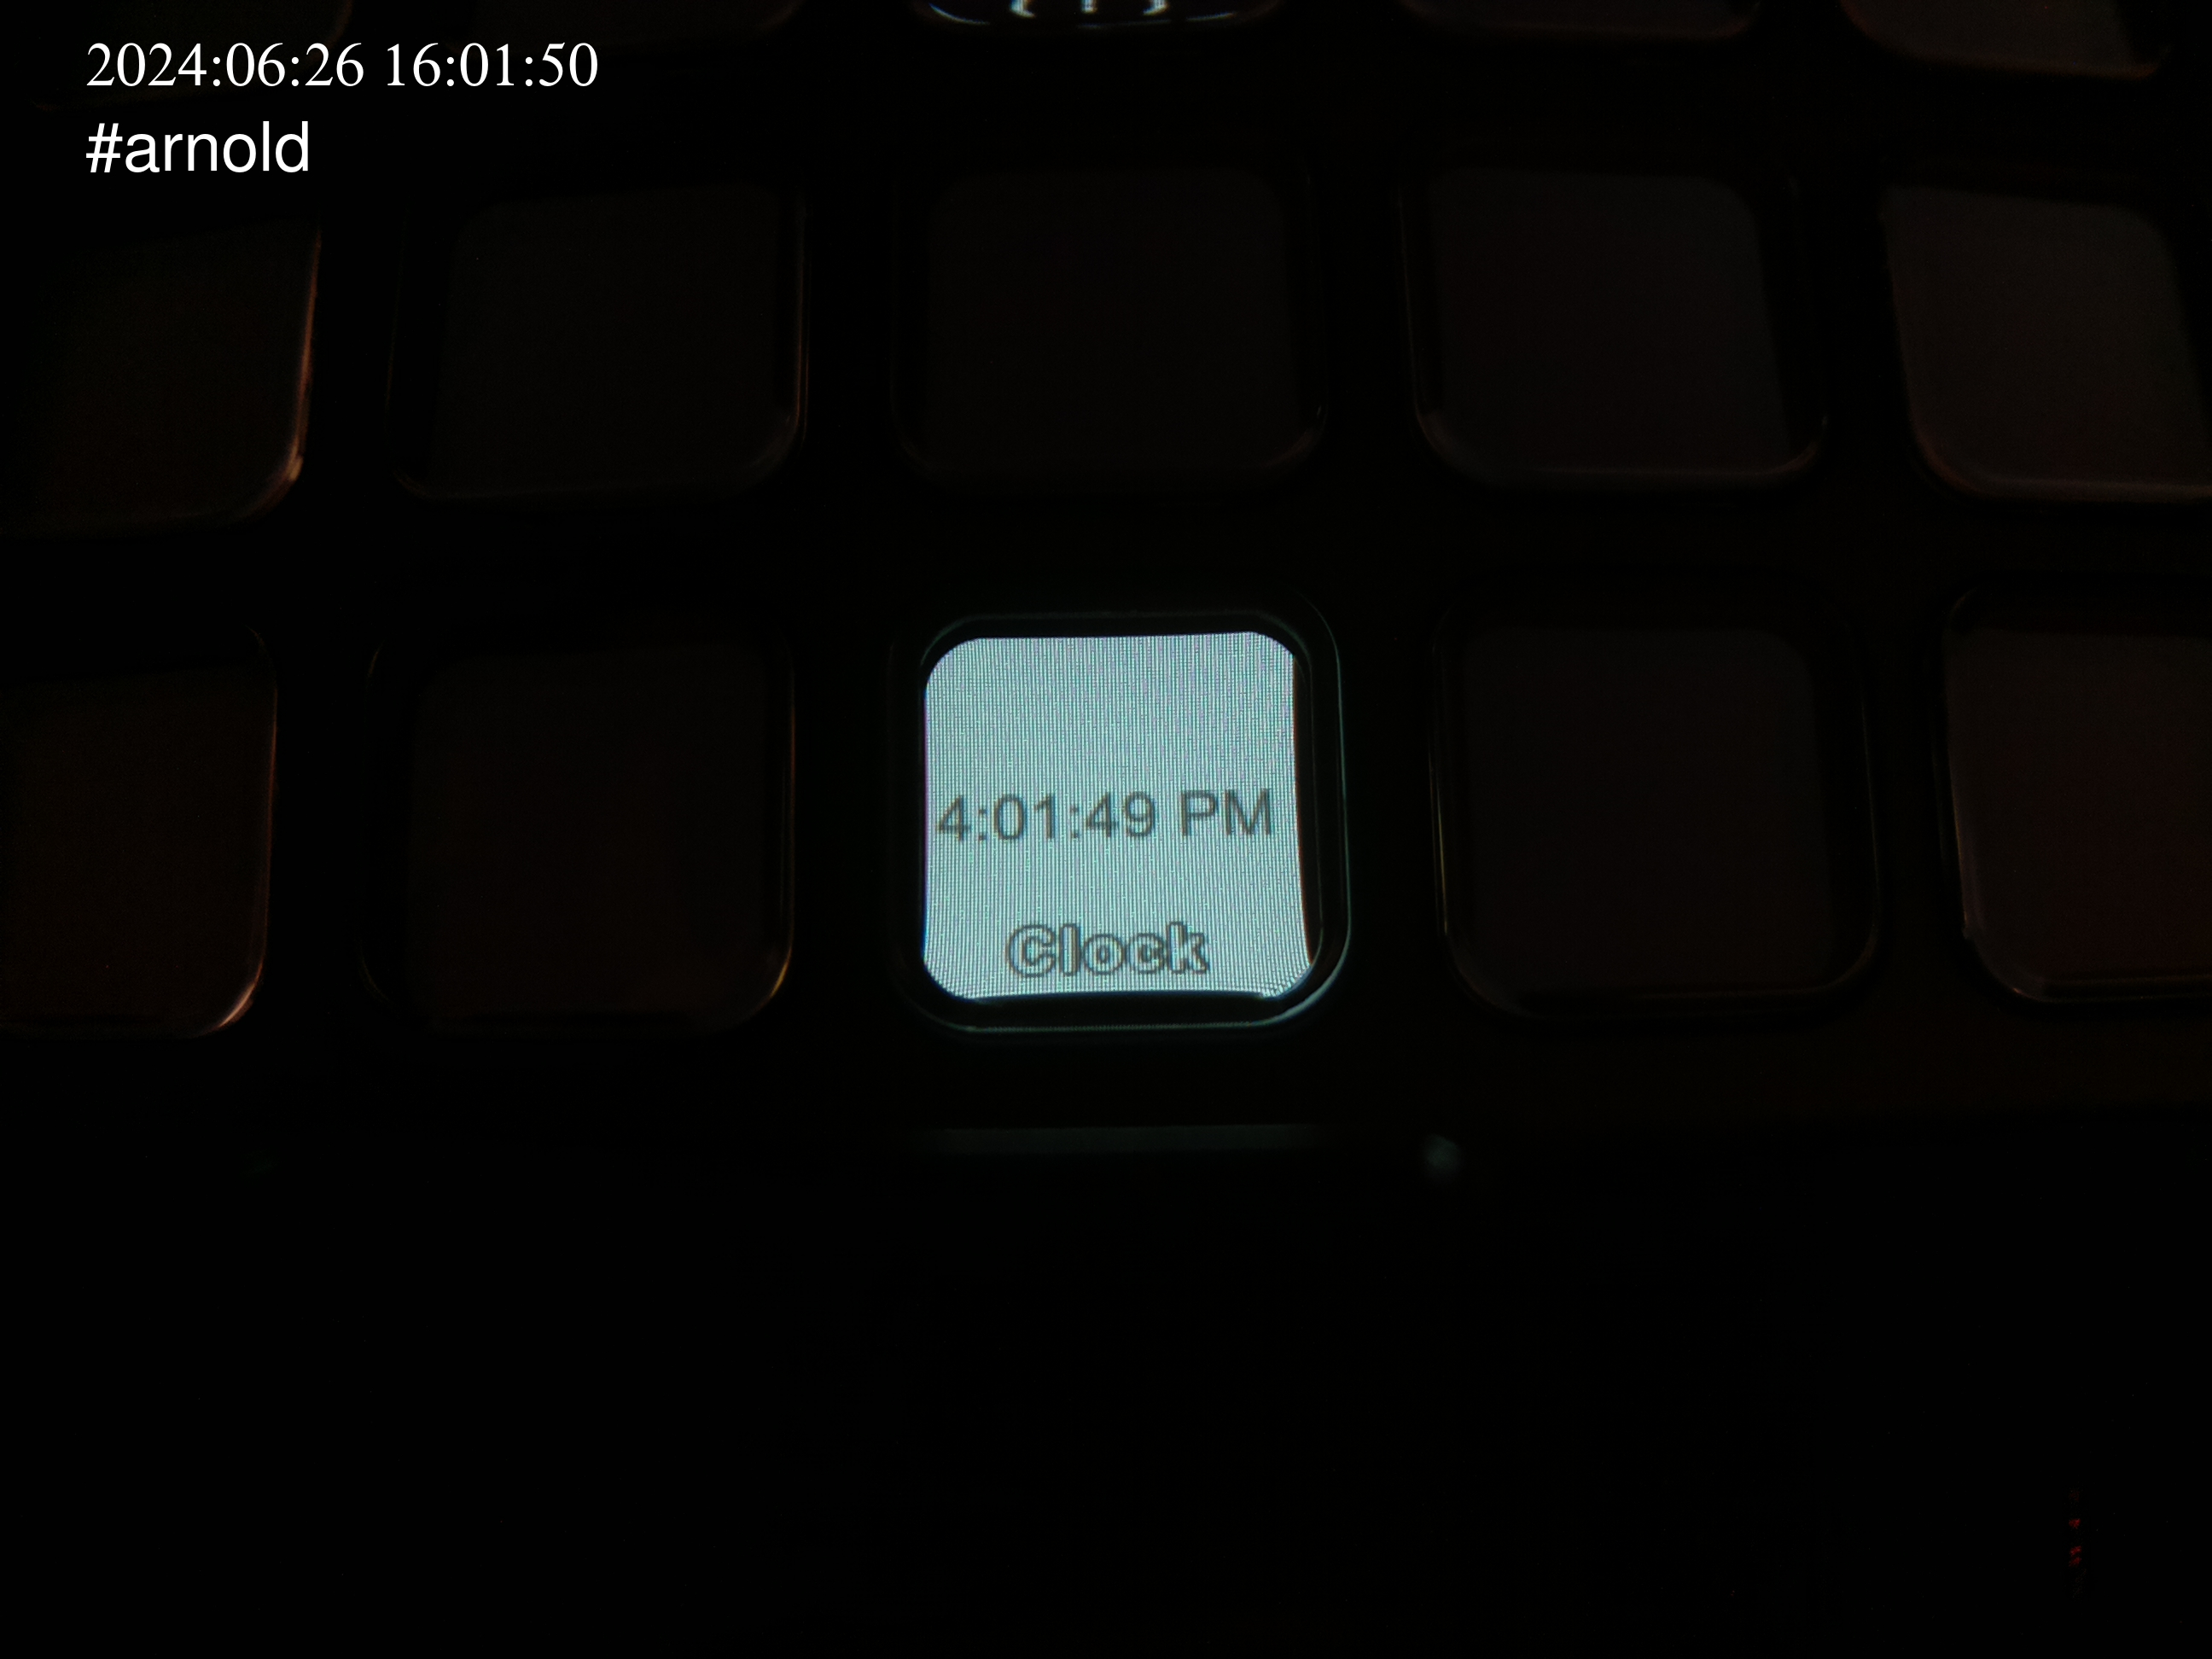
\includegraphics[width=.9\linewidth]{./4.01.jpg}
\end{center}
\section{In Python}
\label{sec:orgda5d379}

\begin{minted}[frame=lines,fontsize=\scriptsize,linenos=]{python}
import requests
import shutil

req = requests.get('http://arnold.wifi.local.cmu.edu:8080/img', stream=True)

img = '4:17.jpg'
with open(img, 'wb') as f:
    req.raw.decode_content = True
    shutil.copyfileobj(req.raw, f)
\end{minted}

\begin{center}
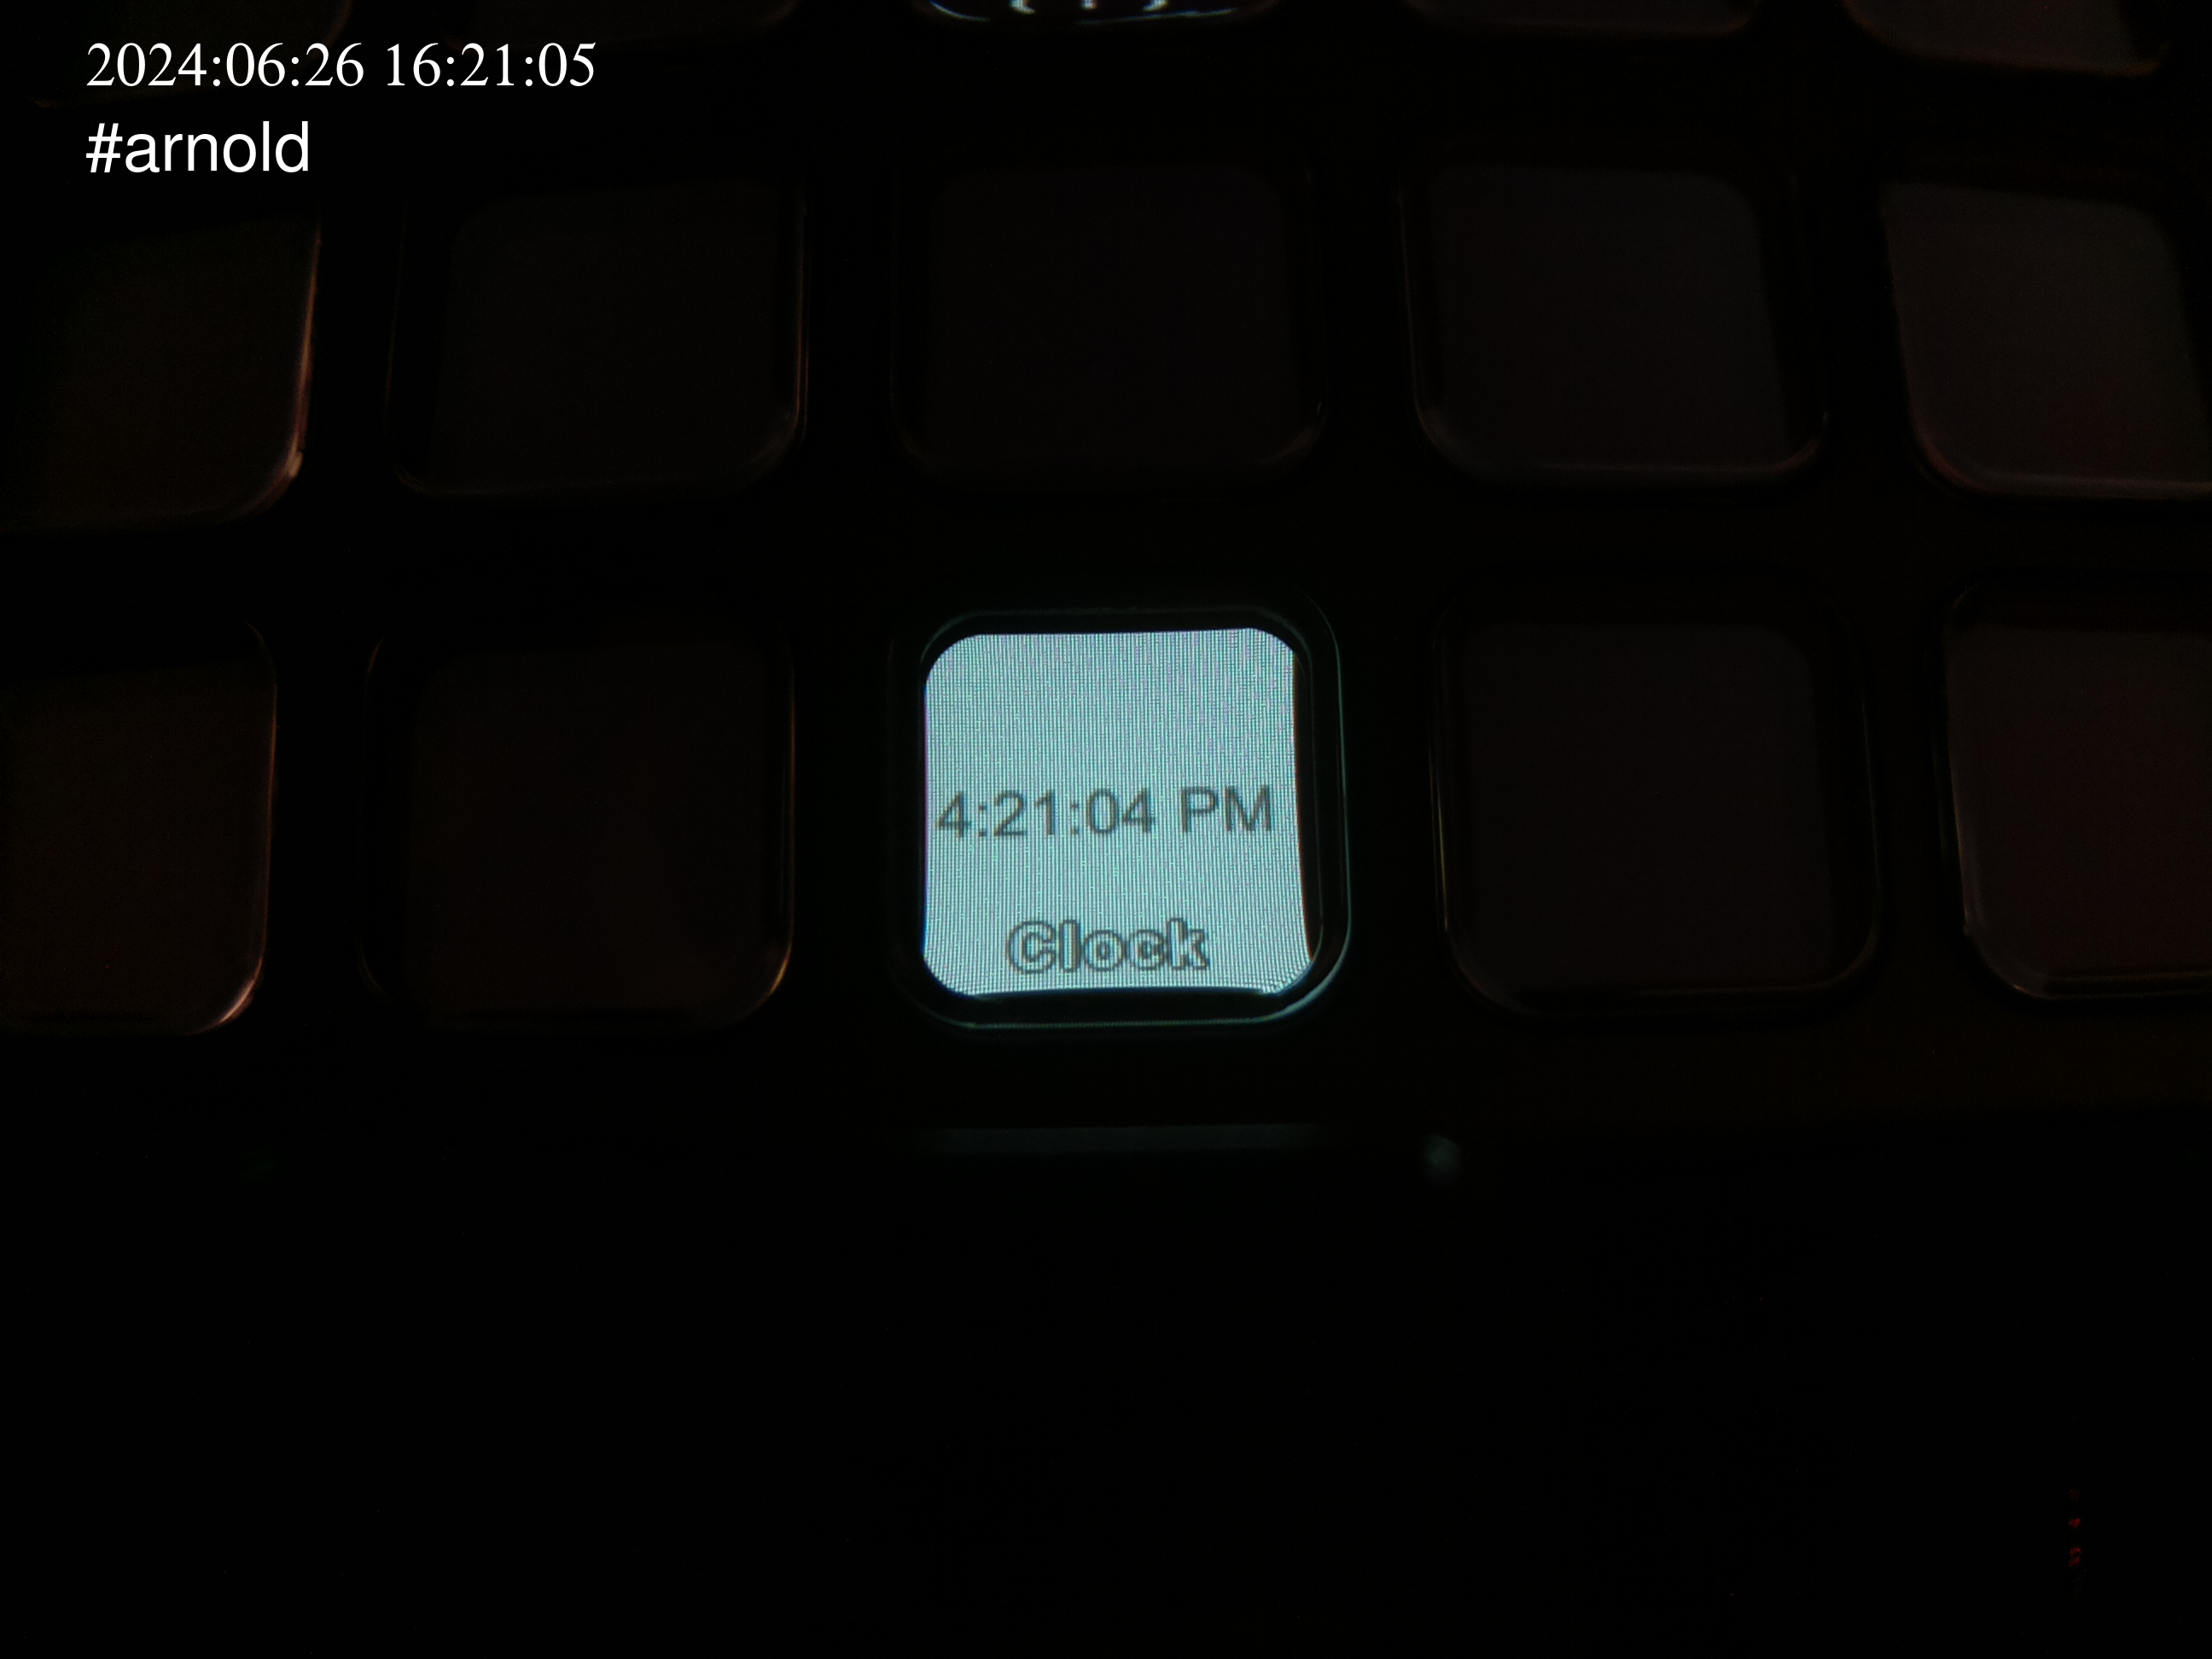
\includegraphics[width=.9\linewidth]{./4:17.jpg}
\end{center}
\section{in elisp}
\label{sec:org46ef293}

\begin{minted}[frame=lines,fontsize=\scriptsize,linenos=]{common-lisp}
(use-package ob-http)

(defun ob-http-file (response filename)
  (let ((body (ob-http-response-body response)))
    (with-temp-file filename
      (insert body)))
  (format "[[%s]]" (expand-file-name filename default-directory)))
\end{minted}

\phantomsection
\label{}
\begin{verbatim}
ob-http-file
\end{verbatim}



\begin{minted}[frame=lines,fontsize=\scriptsize,linenos=]{http}
GET http://arnold.wifi.local.cmu.edu:8080/img
\end{minted}

\begin{center}
\fbox{
\begin{minipage}[c]{.6\linewidth}
\textbf{\textsf{\textsc{DONE}}} there is some font-lock issue

\rule[.8em]{\linewidth}{2pt}

I don't know what it is, something acts sticky, headlines don't always auto format. Something is weird, I thought I updated org, but it looks like I use an old version. It should be 9.7.5.

It was 9.7-pre. still isn't what I thought, but updating might have fixed it?


\begin{minted}[frame=lines,fontsize=\scriptsize,linenos=]{common-lisp}
(org-version)
\end{minted}

\phantomsection
\label{}
\begin{verbatim}
9.7-pre
\end{verbatim}
\end{minipage}
}
\end{center}
\end{document}
